\documentclass[1p]{elsarticle_modified}
%\bibliographystyle{elsarticle-num}

%\usepackage[colorlinks]{hyperref}
%\usepackage{abbrmath_seonhwa} %\Abb, \Ascr, \Acal ,\Abf, \Afrak
\usepackage{amsfonts}
\usepackage{amssymb}
\usepackage{amsmath}
\usepackage{amsthm}
\usepackage{scalefnt}
\usepackage{amsbsy}
\usepackage{kotex}
\usepackage{caption}
\usepackage{subfig}
\usepackage{color}
\usepackage{graphicx}
\usepackage{xcolor} %% white, black, red, green, blue, cyan, magenta, yellow
\usepackage{float}
\usepackage{setspace}
\usepackage{hyperref}

\usepackage{tikz}
\usetikzlibrary{arrows}

\usepackage{multirow}
\usepackage{array} % fixed length table
\usepackage{hhline}

%%%%%%%%%%%%%%%%%%%%%
\makeatletter
\renewcommand*\env@matrix[1][\arraystretch]{%
	\edef\arraystretch{#1}%
	\hskip -\arraycolsep
	\let\@ifnextchar\new@ifnextchar
	\array{*\c@MaxMatrixCols c}}
\makeatother %https://tex.stackexchange.com/questions/14071/how-can-i-increase-the-line-spacing-in-a-matrix
%%%%%%%%%%%%%%%

\usepackage[normalem]{ulem}

\newcommand{\msout}[1]{\ifmmode\text{\sout{\ensuremath{#1}}}\else\sout{#1}\fi}
%SOURCE: \msout is \stkout macro in https://tex.stackexchange.com/questions/20609/strikeout-in-math-mode

\newcommand{\cancel}[1]{
	\ifmmode
	{\color{red}\msout{#1}}
	\else
	{\color{red}\sout{#1}}
	\fi
}

\newcommand{\add}[1]{
	{\color{blue}\uwave{#1}}
}

\newcommand{\replace}[2]{
	\ifmmode
	{\color{red}\msout{#1}}{\color{blue}\uwave{#2}}
	\else
	{\color{red}\sout{#1}}{\color{blue}\uwave{#2}}
	\fi
}

\newcommand{\Sol}{\mathcal{S}} %segment
\newcommand{\D}{D} %diagram
\newcommand{\A}{\mathcal{A}} %arc


%%%%%%%%%%%%%%%%%%%%%%%%%%%%%5 test

\def\sl{\operatorname{\textup{SL}}(2,\Cbb)}
\def\psl{\operatorname{\textup{PSL}}(2,\Cbb)}
\def\quan{\mkern 1mu \triangleright \mkern 1mu}

\theoremstyle{definition}
\newtheorem{thm}{Theorem}[section]
\newtheorem{prop}[thm]{Proposition}
\newtheorem{lem}[thm]{Lemma}
\newtheorem{ques}[thm]{Question}
\newtheorem{cor}[thm]{Corollary}
\newtheorem{defn}[thm]{Definition}
\newtheorem{exam}[thm]{Example}
\newtheorem{rmk}[thm]{Remark}
\newtheorem{alg}[thm]{Algorithm}

\newcommand{\I}{\sqrt{-1}}
\begin{document}

%\begin{frontmatter}
%
%\title{Boundary parabolic representations of knots up to 8 crossings}
%
%%% Group authors per affiliation:
%\author{Yunhi Cho} 
%\address{Department of Mathematics, University of Seoul, Seoul, Korea}
%\ead{yhcho@uos.ac.kr}
%
%
%\author{Seonhwa Kim} %\fnref{s_kim}}
%\address{Center for Geometry and Physics, Institute for Basic Science, Pohang, 37673, Korea}
%\ead{ryeona17@ibs.re.kr}
%
%\author{Hyuk Kim}
%\address{Department of Mathematical Sciences, Seoul National University, Seoul 08826, Korea}
%\ead{hyukkim@snu.ac.kr}
%
%\author{Seokbeom Yoon}
%\address{Department of Mathematical Sciences, Seoul National University, Seoul, 08826,  Korea}
%\ead{sbyoon15@snu.ac.kr}
%
%\begin{abstract}
%We find all boundary parabolic representation of knots up to 8 crossings.
%
%\end{abstract}
%\begin{keyword}
%    \MSC[2010] 57M25 
%\end{keyword}
%
%\end{frontmatter}

%\linenumbers
%\tableofcontents
%
\newcommand\colored[1]{\textcolor{white}{\rule[-0.35ex]{0.8em}{1.4ex}}\kern-0.8em\color{red} #1}%
%\newcommand\colored[1]{\textcolor{white}{ #1}\kern-2.17ex	\textcolor{white}{ #1}\kern-1.81ex	\textcolor{white}{ #1}\kern-2.15ex\color{red}#1	}

{\Large $\underline{12n_{0428}~(K12n_{0428})}$}

\setlength{\tabcolsep}{10pt}
\renewcommand{\arraystretch}{1.6}
\vspace{1cm}\begin{tabular}{m{100pt}>{\centering\arraybackslash}m{274pt}}
\multirow{5}{120pt}{
	\centering
	\includegraphics[width=112pt]{../../../GIT/diagram.site/Diagrams/png/2517_12n_0428.png}\\
\ \ \ A knot diagram\footnotemark}&
\allowdisplaybreaks
\textbf{Linearized knot diagam} \\
\cline{2-2}
 &
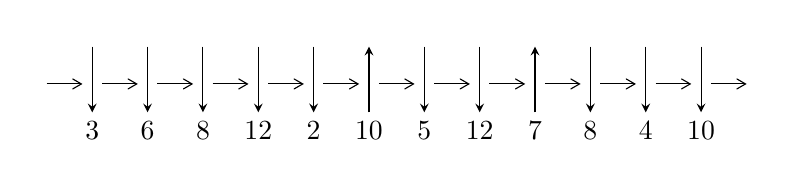
\begin{tikzpicture}[x=20pt, y=17pt]
	% nodes
	\node (C0) at (0, 0) {};
	\node (C1) at (1, 0) {};
	\node (C1U) at (1, +1) {};
	\node (C1D) at (1, -1) {3};

	\node (C2) at (2, 0) {};
	\node (C2U) at (2, +1) {};
	\node (C2D) at (2, -1) {6};

	\node (C3) at (3, 0) {};
	\node (C3U) at (3, +1) {};
	\node (C3D) at (3, -1) {8};

	\node (C4) at (4, 0) {};
	\node (C4U) at (4, +1) {};
	\node (C4D) at (4, -1) {12};

	\node (C5) at (5, 0) {};
	\node (C5U) at (5, +1) {};
	\node (C5D) at (5, -1) {2};

	\node (C6) at (6, 0) {};
	\node (C6U) at (6, +1) {};
	\node (C6D) at (6, -1) {10};

	\node (C7) at (7, 0) {};
	\node (C7U) at (7, +1) {};
	\node (C7D) at (7, -1) {5};

	\node (C8) at (8, 0) {};
	\node (C8U) at (8, +1) {};
	\node (C8D) at (8, -1) {12};

	\node (C9) at (9, 0) {};
	\node (C9U) at (9, +1) {};
	\node (C9D) at (9, -1) {7};

	\node (C10) at (10, 0) {};
	\node (C10U) at (10, +1) {};
	\node (C10D) at (10, -1) {8};

	\node (C11) at (11, 0) {};
	\node (C11U) at (11, +1) {};
	\node (C11D) at (11, -1) {4};

	\node (C12) at (12, 0) {};
	\node (C12U) at (12, +1) {};
	\node (C12D) at (12, -1) {10};
	\node (C13) at (13, 0) {};

	% arrows
	\draw[->,>={angle 60}]
	(C0) edge (C1) (C1) edge (C2) (C2) edge (C3) (C3) edge (C4) (C4) edge (C5) (C5) edge (C6) (C6) edge (C7) (C7) edge (C8) (C8) edge (C9) (C9) edge (C10) (C10) edge (C11) (C11) edge (C12) (C12) edge (C13) ;	\draw[->,>=stealth]
	(C1U) edge (C1D) (C2U) edge (C2D) (C3U) edge (C3D) (C4U) edge (C4D) (C5U) edge (C5D) (C6D) edge (C6U) (C7U) edge (C7D) (C8U) edge (C8D) (C9D) edge (C9U) (C10U) edge (C10D) (C11U) edge (C11D) (C12U) edge (C12D) ;
	\end{tikzpicture} \\
\hhline{~~} \\& 
\textbf{Solving Sequence} \\ \cline{2-2} 
 &
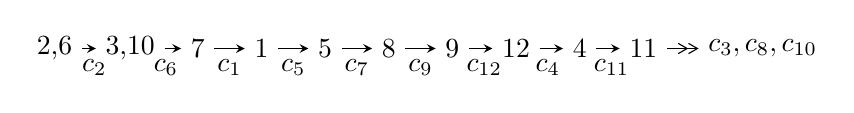
\begin{tikzpicture}[x=23pt, y=7pt]
	% node
	\node (A0) at (-1/8, 0) {2,6};
	\node (A1) at (17/16, 0) {3,10};
	\node (A2) at (17/8, 0) {7};
	\node (A3) at (25/8, 0) {1};
	\node (A4) at (33/8, 0) {5};
	\node (A5) at (41/8, 0) {8};
	\node (A6) at (49/8, 0) {9};
	\node (A7) at (57/8, 0) {12};
	\node (A8) at (65/8, 0) {4};
	\node (A9) at (73/8, 0) {11};
	\node (C1) at (1/2, -1) {$c_{2}$};
	\node (C2) at (13/8, -1) {$c_{6}$};
	\node (C3) at (21/8, -1) {$c_{1}$};
	\node (C4) at (29/8, -1) {$c_{5}$};
	\node (C5) at (37/8, -1) {$c_{7}$};
	\node (C6) at (45/8, -1) {$c_{9}$};
	\node (C7) at (53/8, -1) {$c_{12}$};
	\node (C8) at (61/8, -1) {$c_{4}$};
	\node (C9) at (69/8, -1) {$c_{11}$};
	\node (A10) at (11, 0) {$c_{3},c_{8},c_{10}$};

	% edge
	\draw[->,>=stealth]	
	(A0) edge (A1) (A1) edge (A2) (A2) edge (A3) (A3) edge (A4) (A4) edge (A5) (A5) edge (A6) (A6) edge (A7) (A7) edge (A8) (A8) edge (A9) ;
	\draw[->>,>={angle 60}]	
	(A9) edge (A10);
\end{tikzpicture} \\ 

\end{tabular} \\

\footnotetext{
The image of knot diagram is generated by the software ``\textbf{Draw programme}" developed by Andrew Bartholomew(\url{http://www.layer8.co.uk/maths/draw/index.htm\#Running-draw}), where we modified some parts for our purpose(\url{https://github.com/CATsTAILs/LinksPainter}).
}\phantom \\ \newline 
\centering \textbf{Ideals for irreducible components\footnotemark of $X_{\text{par}}$} 
 
\begin{align*}
I^u_{1}&=\langle 
3309761832986841 u^{28}-484169443496906 u^{27}+\cdots+2728407209023967 b+10346261032522342,\\
\phantom{I^u_{1}}&\phantom{= \langle  }6.12347\times10^{15} u^{28}-3.65447\times10^{15} u^{27}+\cdots+2.72841\times10^{15} a+3.93244\times10^{16},\;u^{29}- u^{28}+\cdots+11 u-1\rangle \\
I^u_{2}&=\langle 
13 u^{13}+7 u^{12}+\cdots+b-29,\;224 u^{13}+105 u^{12}+\cdots+a-480,\\
\phantom{I^u_{2}}&\phantom{= \langle  }u^{14}-5 u^{12}+u^{11}+11 u^{10}-4 u^9-13 u^8+7 u^7+8 u^6-10 u^5- u^4+10 u^3-2 u^2-3 u+1\rangle \\
\\
\end{align*}
\raggedright * 2 irreducible components of $\dim_{\mathbb{C}}=0$, with total 43 representations.\\
\footnotetext{All coefficients of polynomials are rational numbers. But the coefficients are sometimes approximated in decimal forms when there is not enough margin.}
\newpage
\renewcommand{\arraystretch}{1}
\centering \section*{I. $I^u_{1}= \langle 3.31\times10^{15} u^{28}-4.84\times10^{14} u^{27}+\cdots+2.73\times10^{15} b+1.03\times10^{16},\;6.12\times10^{15} u^{28}-3.65\times10^{15} u^{27}+\cdots+2.73\times10^{15} a+3.93\times10^{16},\;u^{29}- u^{28}+\cdots+11 u-1 \rangle$}
\flushleft \textbf{(i) Arc colorings}\\
\begin{tabular}{m{7pt} m{180pt} m{7pt} m{180pt} }
\flushright $a_{2}=$&$\begin{pmatrix}1\\0\end{pmatrix}$ \\
\flushright $a_{6}=$&$\begin{pmatrix}0\\u\end{pmatrix}$ \\
\flushright $a_{3}=$&$\begin{pmatrix}1\\u^2\end{pmatrix}$ \\
\flushright $a_{10}=$&$\begin{pmatrix}-2.24434 u^{28}+1.33942 u^{27}+\cdots+45.0118 u-14.4130\\-1.21307 u^{28}+0.177455 u^{27}+\cdots+17.9088 u-3.79205\end{pmatrix}$ \\
\flushright $a_{7}=$&$\begin{pmatrix}3.72446 u^{28}-1.92791 u^{27}+\cdots-66.8278 u+18.8763\\1.69382 u^{28}-0.176481 u^{27}+\cdots-18.8053 u+4.46366\end{pmatrix}$ \\
\flushright $a_{1}=$&$\begin{pmatrix}- u^2+1\\- u^4\end{pmatrix}$ \\
\flushright $a_{5}=$&$\begin{pmatrix}u\\u\end{pmatrix}$ \\
\flushright $a_{8}=$&$\begin{pmatrix}3.69627 u^{28}-1.96435 u^{27}+\cdots-67.8684 u+19.1555\\1.66563 u^{28}-0.212920 u^{27}+\cdots-19.8460 u+4.74286\end{pmatrix}$ \\
\flushright $a_{9}=$&$\begin{pmatrix}-8.80217 u^{28}+2.99230 u^{27}+\cdots+150.634 u-40.2378\\-5.79123 u^{28}-0.238662 u^{27}+\cdots+64.3246 u-11.6085\end{pmatrix}$ \\
\flushright $a_{12}=$&$\begin{pmatrix}-5.43646 u^{28}+2.41208 u^{27}+\cdots+107.030 u-28.7016\\-2.54933 u^{28}-0.164013 u^{27}+\cdots+33.7253 u-7.14216\end{pmatrix}$ \\
\flushright $a_{4}=$&$\begin{pmatrix}2.50984 u^{28}-6.17071 u^{27}+\cdots-123.703 u+44.9330\\-2.45081 u^{28}-2.07795 u^{27}+\cdots-2.61459 u+7.33026\end{pmatrix}$ \\
\flushright $a_{11}=$&$\begin{pmatrix}11.3793 u^{28}-5.86912 u^{27}+\cdots-218.129 u+62.4454\\6.01027 u^{28}-0.499882 u^{27}+\cdots-76.2473 u+16.4335\end{pmatrix}$\\&\end{tabular}
\flushleft \textbf{(ii) Obstruction class $= -1$}\\~\\
\flushleft \textbf{(iii) Cusp Shapes $= -\frac{29606274479465}{94083007207723} u^{28}-\frac{112181565603524}{94083007207723} u^{27}+\cdots-\frac{79763733552791}{94083007207723} u-\frac{508359165202078}{94083007207723}$}\\~\\
\newpage\renewcommand{\arraystretch}{1}
\flushleft \textbf{(iv) u-Polynomials at the component}\newline \\
\begin{tabular}{m{50pt}|m{274pt}}
Crossings & \hspace{64pt}u-Polynomials at each crossing \\
\hline $$\begin{aligned}c_{1}\end{aligned}$$&$\begin{aligned}
&u^{29}+23 u^{28}+\cdots+57 u+1
\end{aligned}$\\
\hline $$\begin{aligned}c_{2},c_{5}\end{aligned}$$&$\begin{aligned}
&u^{29}+u^{28}+\cdots+11 u+1
\end{aligned}$\\
\hline $$\begin{aligned}c_{3}\end{aligned}$$&$\begin{aligned}
&u^{29}+2 u^{28}+\cdots-512 u-181
\end{aligned}$\\
\hline $$\begin{aligned}c_{4},c_{11}\end{aligned}$$&$\begin{aligned}
&u^{29}+3 u^{28}+\cdots+52 u+17
\end{aligned}$\\
\hline $$\begin{aligned}c_{6},c_{9}\end{aligned}$$&$\begin{aligned}
&u^{29}+6 u^{28}+\cdots-3 u-1
\end{aligned}$\\
\hline $$\begin{aligned}c_{7}\end{aligned}$$&$\begin{aligned}
&u^{29}-3 u^{28}+\cdots-343 u-73
\end{aligned}$\\
\hline $$\begin{aligned}c_{8}\end{aligned}$$&$\begin{aligned}
&u^{29}+3 u^{28}+\cdots-802 u-61
\end{aligned}$\\
\hline $$\begin{aligned}c_{10}\end{aligned}$$&$\begin{aligned}
&u^{29}-2 u^{28}+\cdots+306 u+17
\end{aligned}$\\
\hline $$\begin{aligned}c_{12}\end{aligned}$$&$\begin{aligned}
&u^{29}-13 u^{28}+\cdots-419 u-617
\end{aligned}$\\
\hline
\end{tabular}\\~\\
\newpage\renewcommand{\arraystretch}{1}
\flushleft \textbf{(v) Riley Polynomials at the component}\newline \\
\begin{tabular}{m{50pt}|m{274pt}}
Crossings & \hspace{64pt}Riley Polynomials at each crossing \\
\hline $$\begin{aligned}c_{1}\end{aligned}$$&$\begin{aligned}
&y^{29}-27 y^{28}+\cdots+3781 y-1
\end{aligned}$\\
\hline $$\begin{aligned}c_{2},c_{5}\end{aligned}$$&$\begin{aligned}
&y^{29}-23 y^{28}+\cdots+57 y-1
\end{aligned}$\\
\hline $$\begin{aligned}c_{3}\end{aligned}$$&$\begin{aligned}
&y^{29}-66 y^{28}+\cdots+773288 y-32761
\end{aligned}$\\
\hline $$\begin{aligned}c_{4},c_{11}\end{aligned}$$&$\begin{aligned}
&y^{29}-47 y^{28}+\cdots+3350 y-289
\end{aligned}$\\
\hline $$\begin{aligned}c_{6},c_{9}\end{aligned}$$&$\begin{aligned}
&y^{29}+30 y^{28}+\cdots+5 y-1
\end{aligned}$\\
\hline $$\begin{aligned}c_{7}\end{aligned}$$&$\begin{aligned}
&y^{29}-9 y^{28}+\cdots+108013 y-5329
\end{aligned}$\\
\hline $$\begin{aligned}c_{8}\end{aligned}$$&$\begin{aligned}
&y^{29}-53 y^{28}+\cdots+159352 y-3721
\end{aligned}$\\
\hline $$\begin{aligned}c_{10}\end{aligned}$$&$\begin{aligned}
&y^{29}-74 y^{28}+\cdots+76942 y-289
\end{aligned}$\\
\hline $$\begin{aligned}c_{12}\end{aligned}$$&$\begin{aligned}
&y^{29}-79 y^{28}+\cdots-73773123 y-380689
\end{aligned}$\\
\hline
\end{tabular}\\~\\
\newpage\flushleft \textbf{(vi) Complex Volumes and Cusp Shapes}
$$\begin{array}{c|c|c}  
\text{Solutions to }I^u_{1}& \I (\text{vol} + \sqrt{-1}CS) & \text{Cusp shape}\\
 \hline 
\begin{aligned}
u &= -0.847490 + 0.607947 I \\
a &= -0.422315 - 0.373511 I \\
b &= -0.453967 - 0.141290 I\end{aligned}
 & \phantom{-}1.85694 + 2.41024 I & -0.38198 - 1.83000 I \\ \hline\begin{aligned}
u &= -0.847490 - 0.607947 I \\
a &= -0.422315 + 0.373511 I \\
b &= -0.453967 + 0.141290 I\end{aligned}
 & \phantom{-}1.85694 - 2.41024 I & -0.38198 + 1.83000 I \\ \hline\begin{aligned}
u &= \phantom{-}0.071949 + 0.929488 I \\
a &= \phantom{-}1.55015 + 0.37840 I \\
b &= -0.033988 + 0.404715 I\end{aligned}
 & -5.90516 - 1.34940 I & -11.77988 + 1.16724 I \\ \hline\begin{aligned}
u &= \phantom{-}0.071949 - 0.929488 I \\
a &= \phantom{-}1.55015 - 0.37840 I \\
b &= -0.033988 - 0.404715 I\end{aligned}
 & -5.90516 + 1.34940 I & -11.77988 - 1.16724 I \\ \hline\begin{aligned}
u &= \phantom{-}1.099740 + 0.372987 I \\
a &= \phantom{-}0.429259 - 0.314350 I \\
b &= -0.496131 + 0.172360 I\end{aligned}
 & -2.13143 - 3.61670 I & -10.87499 + 4.53147 I \\ \hline\begin{aligned}
u &= \phantom{-}1.099740 - 0.372987 I \\
a &= \phantom{-}0.429259 + 0.314350 I \\
b &= -0.496131 - 0.172360 I\end{aligned}
 & -2.13143 + 3.61670 I & -10.87499 - 4.53147 I \\ \hline\begin{aligned}
u &= -0.071629 + 1.166630 I \\
a &= -1.42014 + 0.38258 I \\
b &= \phantom{-}0.0590394 - 0.0700190 I\end{aligned}
 & -17.8156 + 5.4788 I & -11.43005 - 2.27554 I \\ \hline\begin{aligned}
u &= -0.071629 - 1.166630 I \\
a &= -1.42014 - 0.38258 I \\
b &= \phantom{-}0.0590394 + 0.0700190 I\end{aligned}
 & -17.8156 - 5.4788 I & -11.43005 + 2.27554 I \\ \hline\begin{aligned}
u &= -1.20779\phantom{ +0.000000I} \\
a &= \phantom{-}1.06012\phantom{ +0.000000I} \\
b &= \phantom{-}0.608535\phantom{ +0.000000I}\end{aligned}
 & -5.45443\phantom{ +0.000000I} & -17.0500\phantom{ +0.000000I} \\ \hline\begin{aligned}
u &= -1.241400 + 0.177721 I \\
a &= \phantom{-}0.09350 - 1.46108 I \\
b &= -0.13368 - 2.49732 I\end{aligned}
 & -4.23135 + 3.90349 I & -13.5060 - 7.1974 I\\
 \hline 
 \end{array}$$\newpage$$\begin{array}{c|c|c}  
\text{Solutions to }I^u_{1}& \I (\text{vol} + \sqrt{-1}CS) & \text{Cusp shape}\\
 \hline 
\begin{aligned}
u &= -1.241400 - 0.177721 I \\
a &= \phantom{-}0.09350 + 1.46108 I \\
b &= -0.13368 + 2.49732 I\end{aligned}
 & -4.23135 - 3.90349 I & -13.5060 + 7.1974 I \\ \hline\begin{aligned}
u &= \phantom{-}0.607700 + 0.416192 I \\
a &= \phantom{-}0.030334 + 0.170685 I \\
b &= \phantom{-}0.768475 - 0.109674 I\end{aligned}
 & -0.645013 + 0.114015 I & -8.30235 - 0.44217 I \\ \hline\begin{aligned}
u &= \phantom{-}0.607700 - 0.416192 I \\
a &= \phantom{-}0.030334 - 0.170685 I \\
b &= \phantom{-}0.768475 + 0.109674 I\end{aligned}
 & -0.645013 - 0.114015 I & -8.30235 + 0.44217 I \\ \hline\begin{aligned}
u &= \phantom{-}1.264620 + 0.097173 I \\
a &= \phantom{-}0.126127 + 0.975567 I \\
b &= \phantom{-}0.45216 + 2.48013 I\end{aligned}
 & -4.42915 + 0.22712 I & -13.77800 + 0.54237 I \\ \hline\begin{aligned}
u &= \phantom{-}1.264620 - 0.097173 I \\
a &= \phantom{-}0.126127 - 0.975567 I \\
b &= \phantom{-}0.45216 - 2.48013 I\end{aligned}
 & -4.42915 - 0.22712 I & -13.77800 - 0.54237 I \\ \hline\begin{aligned}
u &= \phantom{-}1.27084\phantom{ +0.000000I} \\
a &= -2.54450\phantom{ +0.000000I} \\
b &= -2.41619\phantom{ +0.000000I}\end{aligned}
 & -14.6938\phantom{ +0.000000I} & -21.3900\phantom{ +0.000000I} \\ \hline\begin{aligned}
u &= -1.35314\phantom{ +0.000000I} \\
a &= -0.122473\phantom{ +0.000000I} \\
b &= \phantom{-}1.92297\phantom{ +0.000000I}\end{aligned}
 & -15.8953\phantom{ +0.000000I} & -17.3790\phantom{ +0.000000I} \\ \hline\begin{aligned}
u &= \phantom{-}1.288070 + 0.432233 I \\
a &= -0.52667 - 1.40404 I \\
b &= -0.52972 - 2.41614 I\end{aligned}
 & -9.72617 - 3.55628 I & -15.1648 + 2.5004 I \\ \hline\begin{aligned}
u &= \phantom{-}1.288070 - 0.432233 I \\
a &= -0.52667 + 1.40404 I \\
b &= -0.52972 + 2.41614 I\end{aligned}
 & -9.72617 + 3.55628 I & -15.1648 - 2.5004 I \\ \hline\begin{aligned}
u &= -1.36698 + 0.39083 I \\
a &= \phantom{-}0.056520 + 1.082730 I \\
b &= -0.25816 + 2.57538 I\end{aligned}
 & -10.50180 + 6.08146 I & -14.9405 - 3.9753 I\\
 \hline 
 \end{array}$$\newpage$$\begin{array}{c|c|c}  
\text{Solutions to }I^u_{1}& \I (\text{vol} + \sqrt{-1}CS) & \text{Cusp shape}\\
 \hline 
\begin{aligned}
u &= -1.36698 - 0.39083 I \\
a &= \phantom{-}0.056520 - 1.082730 I \\
b &= -0.25816 - 2.57538 I\end{aligned}
 & -10.50180 - 6.08146 I & -14.9405 + 3.9753 I \\ \hline\begin{aligned}
u &= \phantom{-}0.529556\phantom{ +0.000000I} \\
a &= -0.279573\phantom{ +0.000000I} \\
b &= \phantom{-}0.469661\phantom{ +0.000000I}\end{aligned}
 & -0.808015\phantom{ +0.000000I} & -11.9270\phantom{ +0.000000I} \\ \hline\begin{aligned}
u &= \phantom{-}1.43624 + 0.53316 I \\
a &= \phantom{-}0.045983 + 1.342010 I \\
b &= -0.02188 + 2.71357 I\end{aligned}
 & \phantom{-}16.8944 - 11.5066 I & -13.6242 + 4.6544 I \\ \hline\begin{aligned}
u &= \phantom{-}1.43624 - 0.53316 I \\
a &= \phantom{-}0.045983 - 1.342010 I \\
b &= -0.02188 - 2.71357 I\end{aligned}
 & \phantom{-}16.8944 + 11.5066 I & -13.6242 - 4.6544 I \\ \hline\begin{aligned}
u &= -1.40063 + 0.62143 I \\
a &= \phantom{-}0.391966 - 0.973746 I \\
b &= \phantom{-}0.84600 - 2.06054 I\end{aligned}
 & \phantom{-}17.5554 + 0.8894 I & -13.74018 - 0.79352 I \\ \hline\begin{aligned}
u &= -1.40063 - 0.62143 I \\
a &= \phantom{-}0.391966 + 0.973746 I \\
b &= \phantom{-}0.84600 + 2.06054 I\end{aligned}
 & \phantom{-}17.5554 - 0.8894 I & -13.74018 + 0.79352 I \\ \hline\begin{aligned}
u &= -0.024136 + 0.378698 I \\
a &= -2.54654 - 0.61175 I \\
b &= -0.009603 + 0.352025 I\end{aligned}
 & -0.56395 - 1.71430 I & -3.16058 + 4.19709 I \\ \hline\begin{aligned}
u &= -0.024136 - 0.378698 I \\
a &= -2.54654 + 0.61175 I \\
b &= -0.009603 - 0.352025 I\end{aligned}
 & -0.56395 + 1.71430 I & -3.16058 - 4.19709 I \\ \hline\begin{aligned}
u &= \phantom{-}0.128440\phantom{ +0.000000I} \\
a &= -9.72992\phantom{ +0.000000I} \\
b &= -1.96207\phantom{ +0.000000I}\end{aligned}
 & -11.0443\phantom{ +0.000000I} & -5.88640\phantom{ +0.000000I}\\
 \hline 
 \end{array}$$\newpage\newpage\renewcommand{\arraystretch}{1}
\centering \section*{II. $I^u_{2}= \langle 13 u^{13}+7 u^{12}+\cdots+b-29,\;224 u^{13}+105 u^{12}+\cdots+a-480,\;u^{14}-5 u^{12}+\cdots-3 u+1 \rangle$}
\flushleft \textbf{(i) Arc colorings}\\
\begin{tabular}{m{7pt} m{180pt} m{7pt} m{180pt} }
\flushright $a_{2}=$&$\begin{pmatrix}1\\0\end{pmatrix}$ \\
\flushright $a_{6}=$&$\begin{pmatrix}0\\u\end{pmatrix}$ \\
\flushright $a_{3}=$&$\begin{pmatrix}1\\u^2\end{pmatrix}$ \\
\flushright $a_{10}=$&$\begin{pmatrix}-224 u^{13}-105 u^{12}+\cdots-415 u+480\\-13 u^{13}-7 u^{12}+\cdots-29 u+29\end{pmatrix}$ \\
\flushright $a_{7}=$&$\begin{pmatrix}-143 u^{13}-67 u^{12}+\cdots-263 u+304\\67 u^{13}+32 u^{12}+\cdots+129 u-145\end{pmatrix}$ \\
\flushright $a_{1}=$&$\begin{pmatrix}- u^2+1\\- u^4\end{pmatrix}$ \\
\flushright $a_{5}=$&$\begin{pmatrix}u\\u\end{pmatrix}$ \\
\flushright $a_{8}=$&$\begin{pmatrix}-189 u^{13}-89 u^{12}+\cdots-350 u+403\\21 u^{13}+10 u^{12}+\cdots+42 u-46\end{pmatrix}$ \\
\flushright $a_{9}=$&$\begin{pmatrix}-143 u^{13}-67 u^{12}+\cdots-268 u+306\\-8 u^{13}-5 u^{12}+\cdots-25 u+21\end{pmatrix}$ \\
\flushright $a_{12}=$&$\begin{pmatrix}-98 u^{13}-46 u^{12}+\cdots-178 u+210\\-22 u^{13}-10 u^{12}+\cdots-35 u+44\end{pmatrix}$ \\
\flushright $a_{4}=$&$\begin{pmatrix}-130 u^{13}-63 u^{12}+\cdots-249 u+284\\-2 u^{13}-4 u^{12}+\cdots-20 u+12\end{pmatrix}$ \\
\flushright $a_{11}=$&$\begin{pmatrix}62 u^{13}+30 u^{12}+\cdots+114 u-133\\-13 u^{13}-7 u^{12}+\cdots-35 u+31\end{pmatrix}$\\&\end{tabular}
\flushleft \textbf{(ii) Obstruction class $= 1$}\\~\\
\flushleft \textbf{(iii) Cusp Shapes $= 254 u^{13}+120 u^{12}-1214 u^{11}-319 u^{10}+2647 u^9+232 u^8-3201 u^7+272 u^6+2171 u^5-1523 u^4-980 u^3+2088 u^2+476 u-559$}\\~\\
\newpage\renewcommand{\arraystretch}{1}
\flushleft \textbf{(iv) u-Polynomials at the component}\newline \\
\begin{tabular}{m{50pt}|m{274pt}}
Crossings & \hspace{64pt}u-Polynomials at each crossing \\
\hline $$\begin{aligned}c_{1}\end{aligned}$$&$\begin{aligned}
&u^{14}-10 u^{13}+\cdots-13 u+1
\end{aligned}$\\
\hline $$\begin{aligned}c_{2}\end{aligned}$$&$\begin{aligned}
&u^{14}-5 u^{12}+\cdots-3 u+1
\end{aligned}$\\
\hline $$\begin{aligned}c_{3}\end{aligned}$$&$\begin{aligned}
&u^{14}+u^{13}+\cdots+50 u-25
\end{aligned}$\\
\hline $$\begin{aligned}c_{4}\end{aligned}$$&$\begin{aligned}
&u^{14}-2 u^{13}+\cdots-2 u-1
\end{aligned}$\\
\hline $$\begin{aligned}c_{5}\end{aligned}$$&$\begin{aligned}
&u^{14}-5 u^{12}+\cdots+3 u+1
\end{aligned}$\\
\hline $$\begin{aligned}c_{6}\end{aligned}$$&$\begin{aligned}
&u^{14}- u^{13}+\cdots+7 u+1
\end{aligned}$\\
\hline $$\begin{aligned}c_{7}\end{aligned}$$&$\begin{aligned}
&u^{14}+2 u^{13}+\cdots+u-1
\end{aligned}$\\
\hline $$\begin{aligned}c_{8}\end{aligned}$$&$\begin{aligned}
&u^{14}+4 u^{13}+\cdots+2 u+1
\end{aligned}$\\
\hline $$\begin{aligned}c_{9}\end{aligned}$$&$\begin{aligned}
&u^{14}+u^{13}+\cdots-7 u+1
\end{aligned}$\\
\hline $$\begin{aligned}c_{10}\end{aligned}$$&$\begin{aligned}
&u^{14}+15 u^{13}+\cdots+1248 u+169
\end{aligned}$\\
\hline $$\begin{aligned}c_{11}\end{aligned}$$&$\begin{aligned}
&u^{14}+2 u^{13}+\cdots+2 u-1
\end{aligned}$\\
\hline $$\begin{aligned}c_{12}\end{aligned}$$&$\begin{aligned}
&u^{14}+6 u^{13}+\cdots+215 u+25
\end{aligned}$\\
\hline
\end{tabular}\\~\\
\newpage\renewcommand{\arraystretch}{1}
\flushleft \textbf{(v) Riley Polynomials at the component}\newline \\
\begin{tabular}{m{50pt}|m{274pt}}
Crossings & \hspace{64pt}Riley Polynomials at each crossing \\
\hline $$\begin{aligned}c_{1}\end{aligned}$$&$\begin{aligned}
&y^{14}-6 y^{13}+\cdots-45 y+1
\end{aligned}$\\
\hline $$\begin{aligned}c_{2},c_{5}\end{aligned}$$&$\begin{aligned}
&y^{14}-10 y^{13}+\cdots-13 y+1
\end{aligned}$\\
\hline $$\begin{aligned}c_{3}\end{aligned}$$&$\begin{aligned}
&y^{14}-13 y^{13}+\cdots+4600 y+625
\end{aligned}$\\
\hline $$\begin{aligned}c_{4},c_{11}\end{aligned}$$&$\begin{aligned}
&y^{14}-18 y^{13}+\cdots+2 y+1
\end{aligned}$\\
\hline $$\begin{aligned}c_{6},c_{9}\end{aligned}$$&$\begin{aligned}
&y^{14}+7 y^{13}+\cdots-17 y+1
\end{aligned}$\\
\hline $$\begin{aligned}c_{7}\end{aligned}$$&$\begin{aligned}
&y^{14}+8 y^{13}+\cdots+7 y+1
\end{aligned}$\\
\hline $$\begin{aligned}c_{8}\end{aligned}$$&$\begin{aligned}
&y^{14}-16 y^{13}+\cdots-8 y+1
\end{aligned}$\\
\hline $$\begin{aligned}c_{10}\end{aligned}$$&$\begin{aligned}
&y^{14}-9 y^{13}+\cdots-67938 y+28561
\end{aligned}$\\
\hline $$\begin{aligned}c_{12}\end{aligned}$$&$\begin{aligned}
&y^{14}-22 y^{13}+\cdots-5325 y+625
\end{aligned}$\\
\hline
\end{tabular}\\~\\
\newpage\flushleft \textbf{(vi) Complex Volumes and Cusp Shapes}
$$\begin{array}{c|c|c}  
\text{Solutions to }I^u_{2}& \I (\text{vol} + \sqrt{-1}CS) & \text{Cusp shape}\\
 \hline 
\begin{aligned}
u &= -0.835923 + 0.681048 I \\
a &= -0.125313 - 0.206996 I \\
b &= -0.446348 + 0.397563 I\end{aligned}
 & \phantom{-}1.26701 + 2.62945 I & -13.2524 - 5.2108 I \\ \hline\begin{aligned}
u &= -0.835923 - 0.681048 I \\
a &= -0.125313 + 0.206996 I \\
b &= -0.446348 - 0.397563 I\end{aligned}
 & \phantom{-}1.26701 - 2.62945 I & -13.2524 + 5.2108 I \\ \hline\begin{aligned}
u &= \phantom{-}0.345551 + 0.838709 I \\
a &= -1.020240 - 0.715351 I \\
b &= -0.243705 - 0.098495 I\end{aligned}
 & -2.18681 - 1.21939 I & -11.09554 + 1.93458 I \\ \hline\begin{aligned}
u &= \phantom{-}0.345551 - 0.838709 I \\
a &= -1.020240 + 0.715351 I \\
b &= -0.243705 + 0.098495 I\end{aligned}
 & -2.18681 + 1.21939 I & -11.09554 - 1.93458 I \\ \hline\begin{aligned}
u &= -1.22266\phantom{ +0.000000I} \\
a &= \phantom{-}1.67303\phantom{ +0.000000I} \\
b &= \phantom{-}0.728923\phantom{ +0.000000I}\end{aligned}
 & -13.8048\phantom{ +0.000000I} & -11.3860\phantom{ +0.000000I} \\ \hline\begin{aligned}
u &= \phantom{-}1.244710 + 0.138183 I \\
a &= -0.311608 - 0.937054 I \\
b &= \phantom{-}0.34348 - 2.09289 I\end{aligned}
 & -4.37404 - 2.52484 I & -15.1413 + 2.0385 I \\ \hline\begin{aligned}
u &= \phantom{-}1.244710 - 0.138183 I \\
a &= -0.311608 + 0.937054 I \\
b &= \phantom{-}0.34348 + 2.09289 I\end{aligned}
 & -4.37404 + 2.52484 I & -15.1413 - 2.0385 I \\ \hline\begin{aligned}
u &= -0.727304\phantom{ +0.000000I} \\
a &= \phantom{-}1.73201\phantom{ +0.000000I} \\
b &= \phantom{-}2.70193\phantom{ +0.000000I}\end{aligned}
 & -11.7805\phantom{ +0.000000I} & -17.4240\phantom{ +0.000000I} \\ \hline\begin{aligned}
u &= \phantom{-}1.124850 + 0.672854 I \\
a &= \phantom{-}0.314703 + 0.747799 I \\
b &= \phantom{-}0.580657 + 1.233750 I\end{aligned}
 & -4.34890 - 4.36927 I & -12.83000 + 4.03520 I \\ \hline\begin{aligned}
u &= \phantom{-}1.124850 - 0.672854 I \\
a &= \phantom{-}0.314703 - 0.747799 I \\
b &= \phantom{-}0.580657 - 1.233750 I\end{aligned}
 & -4.34890 + 4.36927 I & -12.83000 - 4.03520 I\\
 \hline 
 \end{array}$$\newpage$$\begin{array}{c|c|c}  
\text{Solutions to }I^u_{2}& \I (\text{vol} + \sqrt{-1}CS) & \text{Cusp shape}\\
 \hline 
\begin{aligned}
u &= -1.372300 + 0.328498 I \\
a &= -0.239034 - 1.275240 I \\
b &= -0.26688 - 2.25518 I\end{aligned}
 & -7.44862 + 5.20740 I & -13.30820 - 4.11576 I \\ \hline\begin{aligned}
u &= -1.372300 - 0.328498 I \\
a &= -0.239034 + 1.275240 I \\
b &= -0.26688 + 2.25518 I\end{aligned}
 & -7.44862 - 5.20740 I & -13.30820 + 4.11576 I \\ \hline\begin{aligned}
u &= \phantom{-}0.468087 + 0.001290 I \\
a &= \phantom{-}0.67897 - 1.74706 I \\
b &= -0.682627 - 0.104415 I\end{aligned}
 & -1.36973 - 1.50897 I & -13.46764 + 1.98399 I \\ \hline\begin{aligned}
u &= \phantom{-}0.468087 - 0.001290 I \\
a &= \phantom{-}0.67897 + 1.74706 I \\
b &= -0.682627 + 0.104415 I\end{aligned}
 & -1.36973 + 1.50897 I & -13.46764 - 1.98399 I\\
 \hline 
 \end{array}$$\newpage
\newpage\renewcommand{\arraystretch}{1}
\centering \section*{ III. u-Polynomials}
\begin{tabular}{m{50pt}|m{274pt}}
Crossings & \hspace{64pt}u-Polynomials at each crossing \\
\hline $$\begin{aligned}c_{1}\end{aligned}$$&$\begin{aligned}
&(u^{14}-10 u^{13}+\cdots-13 u+1)(u^{29}+23 u^{28}+\cdots+57 u+1)
\end{aligned}$\\
\hline $$\begin{aligned}c_{2}\end{aligned}$$&$\begin{aligned}
&(u^{14}-5 u^{12}+\cdots-3 u+1)(u^{29}+u^{28}+\cdots+11 u+1)
\end{aligned}$\\
\hline $$\begin{aligned}c_{3}\end{aligned}$$&$\begin{aligned}
&(u^{14}+u^{13}+\cdots+50 u-25)(u^{29}+2 u^{28}+\cdots-512 u-181)
\end{aligned}$\\
\hline $$\begin{aligned}c_{4}\end{aligned}$$&$\begin{aligned}
&(u^{14}-2 u^{13}+\cdots-2 u-1)(u^{29}+3 u^{28}+\cdots+52 u+17)
\end{aligned}$\\
\hline $$\begin{aligned}c_{5}\end{aligned}$$&$\begin{aligned}
&(u^{14}-5 u^{12}+\cdots+3 u+1)(u^{29}+u^{28}+\cdots+11 u+1)
\end{aligned}$\\
\hline $$\begin{aligned}c_{6}\end{aligned}$$&$\begin{aligned}
&(u^{14}- u^{13}+\cdots+7 u+1)(u^{29}+6 u^{28}+\cdots-3 u-1)
\end{aligned}$\\
\hline $$\begin{aligned}c_{7}\end{aligned}$$&$\begin{aligned}
&(u^{14}+2 u^{13}+\cdots+u-1)(u^{29}-3 u^{28}+\cdots-343 u-73)
\end{aligned}$\\
\hline $$\begin{aligned}c_{8}\end{aligned}$$&$\begin{aligned}
&(u^{14}+4 u^{13}+\cdots+2 u+1)(u^{29}+3 u^{28}+\cdots-802 u-61)
\end{aligned}$\\
\hline $$\begin{aligned}c_{9}\end{aligned}$$&$\begin{aligned}
&(u^{14}+u^{13}+\cdots-7 u+1)(u^{29}+6 u^{28}+\cdots-3 u-1)
\end{aligned}$\\
\hline $$\begin{aligned}c_{10}\end{aligned}$$&$\begin{aligned}
&(u^{14}+15 u^{13}+\cdots+1248 u+169)(u^{29}-2 u^{28}+\cdots+306 u+17)
\end{aligned}$\\
\hline $$\begin{aligned}c_{11}\end{aligned}$$&$\begin{aligned}
&(u^{14}+2 u^{13}+\cdots+2 u-1)(u^{29}+3 u^{28}+\cdots+52 u+17)
\end{aligned}$\\
\hline $$\begin{aligned}c_{12}\end{aligned}$$&$\begin{aligned}
&(u^{14}+6 u^{13}+\cdots+215 u+25)(u^{29}-13 u^{28}+\cdots-419 u-617)
\end{aligned}$\\
\hline
\end{tabular}\newpage\renewcommand{\arraystretch}{1}
\centering \section*{ IV. Riley Polynomials}
\begin{tabular}{m{50pt}|m{274pt}}
Crossings & \hspace{64pt}Riley Polynomials at each crossing \\
\hline $$\begin{aligned}c_{1}\end{aligned}$$&$\begin{aligned}
&(y^{14}-6 y^{13}+\cdots-45 y+1)(y^{29}-27 y^{28}+\cdots+3781 y-1)
\end{aligned}$\\
\hline $$\begin{aligned}c_{2},c_{5}\end{aligned}$$&$\begin{aligned}
&(y^{14}-10 y^{13}+\cdots-13 y+1)(y^{29}-23 y^{28}+\cdots+57 y-1)
\end{aligned}$\\
\hline $$\begin{aligned}c_{3}\end{aligned}$$&$\begin{aligned}
&(y^{14}-13 y^{13}+\cdots+4600 y+625)\\
&\cdot(y^{29}-66 y^{28}+\cdots+773288 y-32761)
\end{aligned}$\\
\hline $$\begin{aligned}c_{4},c_{11}\end{aligned}$$&$\begin{aligned}
&(y^{14}-18 y^{13}+\cdots+2 y+1)(y^{29}-47 y^{28}+\cdots+3350 y-289)
\end{aligned}$\\
\hline $$\begin{aligned}c_{6},c_{9}\end{aligned}$$&$\begin{aligned}
&(y^{14}+7 y^{13}+\cdots-17 y+1)(y^{29}+30 y^{28}+\cdots+5 y-1)
\end{aligned}$\\
\hline $$\begin{aligned}c_{7}\end{aligned}$$&$\begin{aligned}
&(y^{14}+8 y^{13}+\cdots+7 y+1)(y^{29}-9 y^{28}+\cdots+108013 y-5329)
\end{aligned}$\\
\hline $$\begin{aligned}c_{8}\end{aligned}$$&$\begin{aligned}
&(y^{14}-16 y^{13}+\cdots-8 y+1)(y^{29}-53 y^{28}+\cdots+159352 y-3721)
\end{aligned}$\\
\hline $$\begin{aligned}c_{10}\end{aligned}$$&$\begin{aligned}
&(y^{14}-9 y^{13}+\cdots-67938 y+28561)\\
&\cdot(y^{29}-74 y^{28}+\cdots+76942 y-289)
\end{aligned}$\\
\hline $$\begin{aligned}c_{12}\end{aligned}$$&$\begin{aligned}
&(y^{14}-22 y^{13}+\cdots-5325 y+625)\\
&\cdot(y^{29}-79 y^{28}+\cdots-73773123 y-380689)
\end{aligned}$\\
\hline
\end{tabular}
\vskip 2pc
\end{document}